\section{Results}
\label{sec:results}
The results below use the post-unblind final-epoch test records for the
predeclared BB1 confirmatory family. Numerical entries are generated from the
append-only study records and retain the distinction between confirmatory and
descriptive analyses.

\subsection{Pilot Epoch Budget}
The validation-only comparison of the predeclared epoch budgets is reported
from the pilot audit artifact. The selected budget, decision interval, and
record-reuse rule are kept separate from the confirmatory accuracy analysis.
The pilot selected the 300-epoch schedule: the paired 300-minus-200
validation interval was $[-0.26,+0.31]$ percentage points and the maximum
predefined low/high-SNR difference was 1.03 percentage points, so the
200-epoch acceptance rule was not met.

\subsection{Post-Unblind Test Performance}
Table~\ref{tab:test-cell-summary} reports the absolute final-epoch test
performance for the six confirmatory cells. Increasing BB1 width from
$0.50\times$ to $1.00\times$ raises accuracy by 1.66 percentage points for
F2 and 1.57 percentage points for F7. Increasing width further to
$2.00\times$ does not improve F2 and reduces the F7 mean relative to
$1.00\times$. The same cell summaries include macro-F1, negative
log-likelihood, and expected calibration error.
\begin{table*}[!t]
\caption{Post-unblind final-epoch test performance and analytical cost by feature geometry and width. Values are means over the 10 split--seed records in each cell; SD is in percentage points. Core FLOPs and preprocessing FLOPs are from the locked ledger.}
\label{tab:test-cell-summary}
\centering
\footnotesize
\setlength{\tabcolsep}{3pt}
\begin{tabular*}{\textwidth}{@{\extracolsep{\fill}}llrrrrrrrrr@{}}
\toprule
Feature & Width & Params & Core FLOPs & Preproc. FLOPs & $n$ & Accuracy (\%) & SD (pp) & Macro-F1 & NLL & ECE \\
\midrule
F2 & 0.50$\times$ & 3,371 & 0.282M & 0.770K & 10 & 60.68 & 0.13 & 0.627 & 1.117 & 0.040 \\
F2 & 1.00$\times$ & 10,987 & 0.974M & 0.770K & 10 & 62.35 & 0.16 & 0.645 & 1.076 & 0.034 \\
F2 & 2.00$\times$ & 38,987 & 3.586M & 0.770K & 10 & 62.20 & 0.17 & 0.642 & 1.084 & 0.027 \\
F7 & 0.50$\times$ & 3,671 & 0.359M & 2.429K & 10 & 60.74 & 0.38 & 0.628 & 1.117 & 0.037 \\
F7 & 1.00$\times$ & 11,587 & 1.127M & 2.429K & 10 & 62.31 & 0.09 & 0.645 & 1.077 & 0.033 \\
F7 & 2.00$\times$ & 40,187 & 3.893M & 2.429K & 10 & 61.57 & 0.28 & 0.633 & 1.106 & 0.032 \\
\bottomrule
\end{tabular*}
\end{table*}

Figure~\ref{fig:feature-capacity-accuracy} shows the record-level values and
the corresponding mean response across the three confirmatory widths.
% Source: analysis/feature_capacity_accuracy_points.csv
% Source CSV SHA-256: E44F0214D00B09C1906DCD13CB08347B71674D55487DFF698E0E76F442BFE946
% Generated by scripts/paper/generate_feature_capacity_figure.py.
\begin{figure}[!t]
\centering
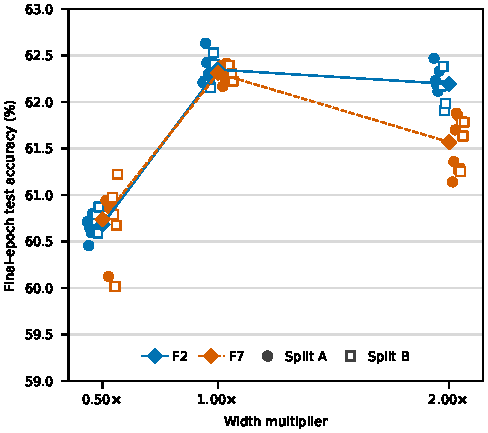
\includegraphics[width=\columnwidth]{feature_capacity_accuracy.pdf}
\xdef\xfigwd{\the\columnwidth}
\caption{Final-epoch test accuracy across the confirmatory width conditions. Each point is one split--seed record ($n=10$ per cell); circles and squares indicate Split A and Split B, respectively. Lines connect cell means. Statistical contrasts are computed from paired split--seed differences and are reported in Table~\ref{tab:confirmatory-statistics}.}
\label{fig:feature-capacity-accuracy}
\end{figure}


\subsection{Feature and Capacity Contrasts}
The complete confirmatory family is reported in
Table~\ref{tab:confirmatory-statistics}. Feature contrasts are F7 minus F2,
capacity contrasts are larger width minus smaller width, and the interaction
is the F7 capacity effect minus the F2 capacity effect. Exact two-sided
sign-permutation $p$-values are Holm-corrected across the 10 contrasts.
With $n=10$ paired split--seed units, the smallest attainable two-sided
$p$-value is $2/2^{10}=0.001953$, reported as 0.0020 when rounded.
Differences in the text and table were computed from unrounded records; the
displayed cell means are rounded.
At $2.00\times$, F7 is lower than F2 by 0.63 percentage points
(Holm-adjusted $p=0.0195$), whereas the feature contrasts at $0.50\times$
and $1.00\times$ are not distinguishable under this protocol. The
$0.50\times$--$1.00\times$ capacity increase is positive for both feature
sets, while the $1.00\times$--$2.00\times$ change is not distinguishable for
F2 and is negative for F7. The global interaction contrast is
$-0.68$ percentage points (Holm-adjusted $p=0.0312$).
The ten paired contrasts are visualized in Fig.~\ref{fig:confirmatory-test-effects}.
\begin{table*}[!t]
\caption{Post-unblind test feature--capacity contrasts. Intervals are paired $t$ 95\% intervals; raw sign-permutation $p$-values are Holm-corrected over the 10 confirmatory contrasts. Here, $d_z=\bar d/s_d$ is the standardized mean paired difference, and $n=10$ split--seed units.}
\label{tab:confirmatory-statistics}
\centering
\footnotesize
\begin{tabular*}{\textwidth}{@{\extracolsep{\fill}}ll>{\centering\arraybackslash}c>{\centering\arraybackslash}c>{\centering\arraybackslash}c>{\centering\arraybackslash}c>{\centering\arraybackslash}c l@{}}
\toprule
Contrast & Unit & Estimate (pp) & 95\% interval & $d_z$ & Raw $p$ & Holm $p$ & Decision \\
\midrule
F7--F2 at $0.50\times$ & split--seed & $+0.05$ & $[-0.23, +0.34]$ & 0.14 & 0.6738 & 1.0000 & Not distinguishable \\
F7--F2 at $1.00\times$ & split--seed & $-0.04$ & $[-0.18, +0.10]$ & $-0.21$ & 0.5137 & 1.0000 & Not distinguishable \\
F7--F2 at $2.00\times$ & split--seed & $-0.63$ & $[-0.89, -0.36]$ & $-1.71$ & 0.0020 & 0.0195 & F7 lower \\
F2: $0.50$--$2.00\times$ & split--seed & $+1.51$ & $[+1.37, +1.65]$ & 7.63 & 0.0020 & 0.0195 & Positive \\
F7: $0.50$--$2.00\times$ & split--seed & $+0.83$ & $[+0.45, +1.21]$ & 1.55 & 0.0020 & 0.0195 & Positive \\
F2: $0.50$--$1.00\times$ & split--seed & $+1.66$ & $[+1.52, +1.81]$ & 8.17 & 0.0020 & 0.0195 & Positive \\
F2: $1.00$--$2.00\times$ & split--seed & $-0.15$ & $[-0.35, +0.05]$ & $-0.55$ & 0.1055 & 0.3164 & Not distinguishable \\
F7: $0.50$--$1.00\times$ & split--seed & $+1.57$ & $[+1.28, +1.86]$ & 3.86 & 0.0020 & 0.0195 & Positive \\
F7: $1.00$--$2.00\times$ & split--seed & $-0.74$ & $[-0.97, -0.52]$ & $-2.37$ & 0.0020 & 0.0195 & Negative \\
Interaction (F7--F2 capacity effect) & split--seed & $-0.68$ & $[-1.09, -0.27]$ & $-1.18$ & 0.0078 & 0.0312 & Negative \\
\bottomrule
\end{tabular*}
\end{table*}


\begin{figure*}[!t]
\centering
\includegraphics[width=0.75\textwidth]{confirmatory_test_effects.pdf}
% The local IEEE Access class expects this width marker for ordinary figures.
\xdef\xfigwd{\the\textwidth}
\caption{Post-unblind test contrasts. Bars are paired 95\% $t$ intervals;
filled markers indicate Holm-adjusted $p<0.05$. The shaded band marks
$\pm0.15$ percentage points.}
\label{fig:confirmatory-test-effects}
\end{figure*}


\subsection{Split-Stratified Sensitivity}
Table~\ref{tab:split-sensitivity} gives split-stratified test
contrasts. The direction of the $2.00\times$ F7--F2 contrast is the same in
both splits, as is the direction of the F7 $1.00\times$--$2.00\times$
contrast. These split-specific values are descriptive consistency checks;
they are not treated as an additional independent inferential family.
\begin{table}[!t]
\caption{Split-stratified sensitivity checks for all 10 confirmatory test contrasts. These values are descriptive consistency checks, not an additional inferential family.}
\label{tab:split-sensitivity}
\centering
\footnotesize
\setlength{\tabcolsep}{3pt}
\begin{tabular*}{\columnwidth}{@{\extracolsep{\fill}}lccc@{}}
\toprule
Contrast & Split A (pp) & Split B (pp) & $n$ per split \\
\midrule
F7--F2 at 0.50$\times$ & $+0.10$ & $+0.01$ & 5 \\
F7--F2 at 1.00$\times$ & $-0.05$ & $-0.03$ & 5 \\
F7--F2 at 2.00$\times$ & $-0.68$ & $-0.58$ & 5 \\
F2: 0.50$\times$--1.00$\times$ & $+1.72$ & $+1.61$ & 5 \\
F2: 0.50$\times$--2.00$\times$ & $+1.62$ & $+1.40$ & 5 \\
F2: 1.00$\times$--2.00$\times$ & $-0.09$ & $-0.21$ & 5 \\
F7: 0.50$\times$--1.00$\times$ & $+1.57$ & $+1.57$ & 5 \\
F7: 0.50$\times$--2.00$\times$ & $+0.84$ & $+0.81$ & 5 \\
F7: 1.00$\times$--2.00$\times$ & $-0.72$ & $-0.76$ & 5 \\
Interaction (F7--F2) & $-0.78$ & $-0.59$ & 5 \\
\bottomrule
\end{tabular*}
\end{table}

The pre-unblind validation analysis gave the same contrast directions and the
same Holm decisions. It is treated as a protocol-consistency check rather than
as additional test evidence.
